
\documentclass{article}

\usepackage{hyperref}
\usepackage{listings}
\usepackage{graphicx}
\newcommand{\email}[1]{\href{mailto:#1}{#1}}

\newcommand{\sql}[1]{\lstinputlisting[language=sql]{sql/#1.sql}}


\title{
  Database Design Project\\
  IT 30
}
\author{
  Samuel Grahn, \email{samuel.grahn@outlook.com}\\
  Olof Bergenholtz, \email{obergenholtz@gmail.com}\\
  Masood Ahmed Rafay, \email{Rafayqureshi2010@gmail.com}\\
  Ali Kamran, \email{alkmrn1@gmail.com}\\
}

\begin{document}

\maketitle
\newpage
\section*{ER-diagram}
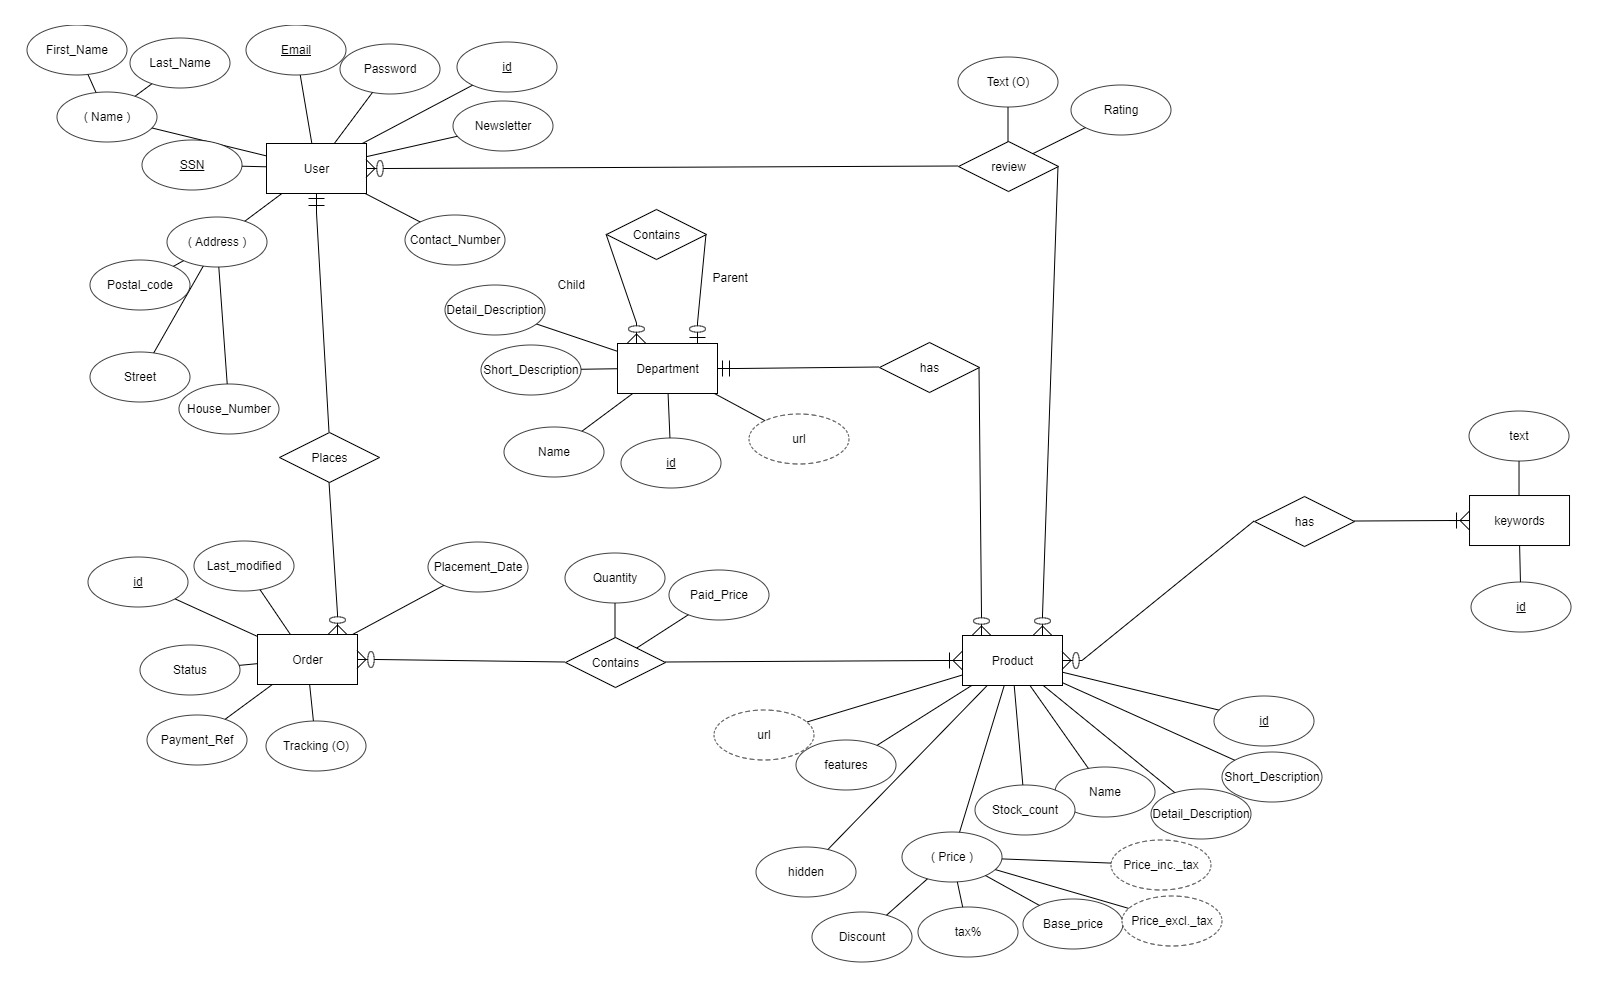
\includegraphics[height=\linewidth,angle=90]{er.png}

\section*{Generating the Database}
\sql{table_generation}

\section*{Task 4 Queries}
Welcome Text
\sql{welcome}
List of top-level departments
\sql{topleveldpt}
List of featured products
\sql{featured_products}
List all keyword-related producs to a product
\sql{similar_products}
List all products in a given department
\sql{dept_products}
List all products on sale sorted by discount percentage
\sql{sale}

\section*{Task 5 Indices}
To improve the query for featured products, we create an index using\\
\sql{indices}

Running
\sql{explain}
before and after creating this index yields\\
\begin{tabular}{ | c c c c c c c c c c | }
  \hline
  id & select\_type & table & type & possible\_keys & key & key\_len & ref & rows & extra\\
  \hline
  1 & SIMPLE & products & ALL & NULL & NULL & NULL & NULL & 11 & Using where\\
  1 & SIMPLE & products & ref & featured\_idx & featured\_idx & 2 & const & 5 & NULL\\
  \hline
\end{tabular}

\section*{Task 6 Questions}

\section{Table relations and FDs}

\subsection{User(id, ssn, email, password, name, address, contact\_no)}

candidate keys: {id}, {ssn}, {email}

name is a composite attribute of first\_name and last\_name



address is a composite attribute of street, house\_number and postal\_code


Functional dependency:\\\\

id $\rightarrow$ ssn, email, password, name, address, contact\_no

ssn $\rightarrow$ id, email, password, name, address, contact\_no

email $\rightarrow$ id, ssn, password, name, address, contact\_no

Normalization: It is not 1NF since we are using composite attributes name and address. Since 1NF is not upheld, neither is 2NF or 3NF.



\section{Product(id, name, url, price, stock\_count, short\_desc, detailed\_desc, features, hidden)}

candidate key: {id}

price is a composite attribute of discount, tax, base\_price, price\_excl\_tax, price\_incl\_tax



Functional dependency:

id $\rightarrow$ name, url, price, stock\_count, short\_desc, detailed\_desc, features, hidden


short\_desc $\rightarrow$ detailed\_desc


base\_price $\rightarrow$ price, price\_excl\_tax,
price\_incl\_tax


tax  $\rightarrow$ price, price\_incl\_tax

Normalization: It is not 1NF since we are using composite attributes name and address. Since 1NF is not upheld, neither is 2NF or 3NF.




\section{Review(product\_id, user\_id, text, rating)}


candidate key: {product\_id, user\_id}

product\_id and user\_id are foreign keys.


Functional dependency:

product\_id, user\_id $\rightarrow$ text, rating

Normalization: It is not 1NF since text is not atomic. Since 1NF is not upheld, neither is 2NF or 3NF.

\end{document}
